% !TEX root = main.tex
% Main text: abstract through conclusion. Formal assumptions, full statements and proofs are in the appendix.
\begin{abstract}
Counting how often a letter occurs, modulo a small number, is easy to learn from the running counts and hard to learn
from the final count alone, although one Transformer can execute either format exactly. We explain the gap by gradient
credit resolved by interaction degree: an interaction among several letters receives credit only from the matching part of
the model's Jacobian. Every letter the final count hides shrinks its low-degree parts by a factor $\mixrate<1$, while a
freshly initialized Transformer is sensitive almost only to low-degree features; a running count depends on the displayed
count and one letter, and pays its cost once. For a two-block Transformer holding exact executors for both formats, outcome
gradient flow from a zero readout stays near chance for a time exponential in the number of letters. With a gate head that
reads the displayed count and the current letter, joint gradient flow on the running counts, from small random magnitudes
along the directions of a hand-coded gate, predicts every count $s_t$, $t\ge2$, correctly after a time polynomial in the
initialization scale and, at fixed head dimension, independent of the number of letters. In experiments, outcome training learns the low-degree prior and almost
nothing beyond it, and step supervision also helps on other state-tracking tasks and with LoRA-tuned Qwen2.5-0.5B on
BIG-Bench Hard object tracking, though not at every size.
\end{abstract}

% ===================================================================
\section{Introduction}
\label{sec:intro}

Training a model on intermediate steps, rather than on final answers alone, often makes reasoning tasks learnable
\citep{nye2021scratchpads,wei2022cot,lightman2023verify}. Why it helps is less clear: in many cases the same network can
represent the answer-only solution, so the difference lies in optimization, not capacity.

We study this question on the simplest task where it arises sharply: counting a query letter modulo $K$. The model
either predicts the final count alone (\emph{outcome supervision}) or every running count as well (\emph{step
supervision}, \cref{fig:chain}b). With the same architecture, initialization, data and budget, outcome training stays
at chance while step training solves the task (\cref{fig:overview}a), even though one two-block Transformer holds an
exact executor for each format (\cref{prop:represent}).

Our explanation is a mismatch between where the target's signal lies and what a freshly initialized network can feel.
Decompose the answer by the number of letters each part depends on jointly, its interaction degree. Every letter the
answer hides contracts its low-degree parts by a factor $\mixrate<1$, so a long answer lives almost entirely at high
degree. A Transformer near initialization has a Jacobian concentrated at degrees $0$ and $1$ (\cref{fig:overview}b), and
the gradient pairs only matching degrees. A running count, by contrast, depends on the displayed count and one letter, so
its signal sits at degree two with no exponential horizon penalty. The two causal chains are
\[
\begin{aligned}
 &\text{outcome:}&&\text{hidden letters}\to\text{high-degree target}\to\text{low Jacobian overlap}\to\text{tiny credit}\to\text{plateau},\\
 &\text{step:}&&\text{displayed count}\to\text{local innovation}\to\text{accessible credit}\to\text{learned transition}\to\text{solution}.
\end{aligned}
\]

\begin{figure}[t]
\centering
%% Figure 1 (pgfplots). Data: results/paper/zero_readout_n16_8k (seeds 42-51, median and 25th-75th percentile band),
%% results/paper/fig2/n8_s42.json (target A_r) and results/paper/exact_spectra/sigma_sweep/s42_sg0.02.txt (Jacobian J_r).
\definecolor{stepc}{HTML}{0072B2}\definecolor{outc}{HTML}{D55E00}\definecolor{theoc}{HTML}{009E73}
\definecolor{modelc}{HTML}{7B4F9E}\definecolor{mutedc}{HTML}{6E6E6E}
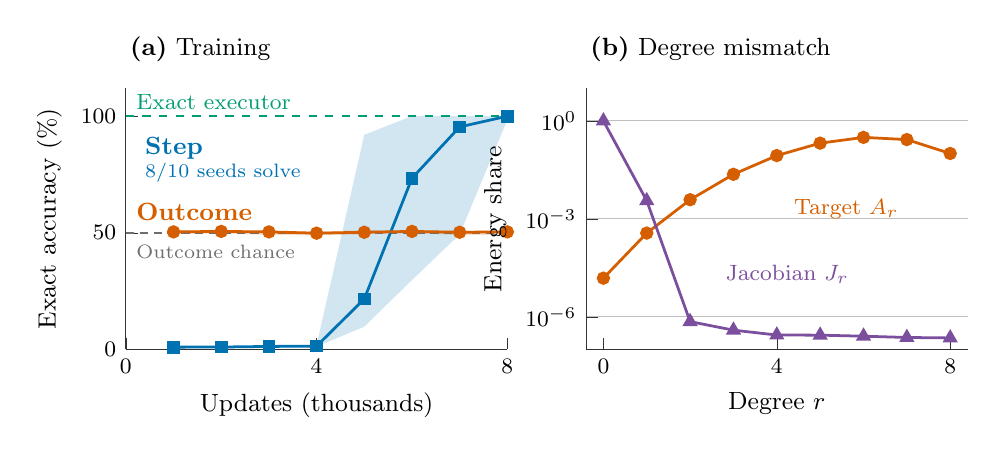
\begin{tikzpicture}
\pgfplotsset{every axis/.style={width=0.53\linewidth, height=4.9cm, axis line style={black!80}, tick style={black!80},
  tick label style={font=\footnotesize}, label style={font=\small}, title style={font=\small, at={(0,1)}, anchor=south west, xshift=-2pt}},
  every axis plot/.append style={line width=1pt}}
\begin{axis}[name=train, title={\textbf{(a)} Training}, xlabel={Updates (thousands)}, ylabel={Exact accuracy (\%)},
  xmin=0, xmax=8, ymin=0, ymax=112, xtick={0,4,8}, ytick={0,50,100}, axis x line*=bottom, axis y line*=left, clip=false]
  \addplot[draw=none, fill=stepc, fill opacity=0.18, forget plot] coordinates {(1,0.55) (2,0.73) (3,0.82) (4,1.25) (5,9.77) (6,29.75) (7,49.33) (8,98.40) (8,100.00) (7,100.00) (6,100.00) (5,92.03) (4,1.90) (3,1.40) (2,1.35) (1,1.35)};
  \addplot[draw=none, fill=outc, fill opacity=0.18, forget plot] coordinates {(1,49.52) (2,49.73) (3,49.05) (4,48.92) (5,49.35) (6,49.92) (7,48.97) (8,49.15) (8,50.70) (7,50.70) (6,51.20) (5,51.08) (4,50.60) (3,50.70) (2,51.08) (1,51.08)};
  \addplot[theoc, dashed, line width=0.9pt, domain=0:8, samples=2] {100};
  \addplot[mutedc, densely dashed, line width=0.8pt, domain=0:8, samples=2] {50};
  \addplot[stepc, mark=square*, mark size=1.8pt] coordinates {(1,1.00) (2,1.05) (3,1.30) (4,1.45) (5,21.65) (6,73.40) (7,95.40) (8,100.00)};
  \addplot[outc, mark=*, mark size=1.9pt] coordinates {(1,50.40) (2,50.60) (3,50.40) (4,49.85) (5,50.25) (6,50.60) (7,50.25) (8,50.40)};
  \node[anchor=south west, font=\footnotesize, text=theoc, inner sep=1pt] at (axis cs:0.15,101.5) {Exact executor};
  \node[anchor=west, font=\small\bfseries, text=stepc] at (axis cs:0.2,86) {Step};
  \node[anchor=west, font=\scriptsize, text=stepc] at (axis cs:0.2,76) {8/10 seeds solve};
  \node[anchor=south west, font=\small\bfseries, text=outc, inner sep=1pt] at (axis cs:0.15,54) {Outcome};
  \node[anchor=north west, font=\scriptsize, text=mutedc, inner sep=1pt] at (axis cs:0.15,46) {Outcome chance};
\end{axis}
\begin{semilogyaxis}[at={(train.east)}, anchor=west, xshift=1.0cm, title={\textbf{(b)} Degree mismatch}, xlabel={Degree $r$},
  ylabel={Energy share}, xmin=-0.4, xmax=8.4, ymin=1e-7, ymax=10, xtick={0,4,8}, ytick={1e-6,1e-3,1},
  ymajorgrids, major grid style={black!25}, axis x line*=bottom, axis y line*=left]
  \addplot[outc, mark=*, mark size=1.9pt] coordinates {(0,1.5259e-05) (1,3.6621e-04) (2,3.8452e-03) (3,2.3071e-02) (4,8.6517e-02) (5,2.0764e-01) (6,3.1146e-01) (7,2.6697e-01) (8,1.0011e-01)};
  \addplot[modelc, mark=triangle*, mark size=2.2pt] coordinates {(0,9.9641e-01) (1,3.5840e-03) (2,7.1281e-07) (3,3.9081e-07) (4,2.7680e-07) (5,2.7450e-07) (6,2.5510e-07) (7,2.3310e-07) (8,2.2560e-07)};
  \node[anchor=north, font=\footnotesize, text=outc] at (axis cs:5.6,8e-3) {Target $A_r$};
  \node[anchor=west, font=\footnotesize, text=modelc] at (axis cs:2.6,2e-5) {Jacobian $J_r$};
\end{semilogyaxis}
\end{tikzpicture}

\caption{\textbf{Same architecture and task, different training behavior.}
(a)~Counting with $n=16$, $K=2$ and zero readout: median exact continuation accuracy and interquartile band over ten paired seeds, $8$k
updates; the dashed line marks the exact executor that both formats admit (\cref{prop:represent}).
(b)~A separate $n=8$, $K=2$, $\initscale=0.02$ measurement with nonzero readout: target and Jacobian energy occupy different degrees (\cref{app:spectrum}).}
\label{fig:overview}
\end{figure}

\paragraph{Contributions.}
\begin{itemize}[leftmargin=*,itemsep=2pt,topsep=3pt]
\item \textbf{Credit is resolved by degree} (\cref{sec:credit}). The gradient of any loss pairs each degree of the
target with the same degree of the Jacobian. Outcome interaction credit decays like $\mixrate^n$; the upper bound and leading coefficient of step credit
for the counting rule carry no such factor (\cref{thm:main,thm:separation}).
\item \textbf{Outcome training plateaus} (\cref{thm:outcome-end}). From a zero readout, gradient flow stays near chance under any block schedule, the relative bias included,
for time $\Omega(\mixrate^{-n})$, in a Transformer wide enough to hold the outcome executor.
\item \textbf{Step training converges} (\cref{thm:joint}). For a gate head that reads the displayed count and the current
letter, joint gradient flow on its query, key and both readouts, from small random magnitudes along hand-coded directions,
reaches positive margins on every count in a time polynomial in the initialization scale and the head dimension, with no other dependence on $n$.
\item \textbf{Experiments} (\cref{sec:experiments}) test each prediction: the exponential plateau, outcome accuracy at the
low-degree prior, learnable routing, and step supervision beyond counting, including a pretrained model.
\end{itemize}

Unlike work on the learnability of parity, we ask why one supervision format succeeds and the other fails for one fixed
target in one model; \cref{sec:related} discusses the relation in detail.

% ===================================================================
\section{Setup}
\label{sec:setup}
\label{sec:setting}

\begin{definition}[Counting modulo $K$]
\label{def:task}
A prompt has a start count $s_0$, uniform on $\mathbb Z_K$, and letters $w_1,\ldots,w_n$ drawn i.i.d.\ from an alphabet
in which a fixed query letter $w^\star$ has probability $p\in(0,1)$. With $b_t=\mathbf 1[w_t=w^\star]$,
\begin{equation}
 s_t=s_{t-1}+b_t\pmod K,\qquad t=1,\ldots,n,
 \label{eq:tracking}
\end{equation}
and the answer is $y=s_n$.
\end{definition}

\begin{definition}[Contraction coefficient]
\label{def:lambda}
For counting modulo $K$,
\begin{equation}
 \mixrate=\max_{1\le j<K}\bigl|1-p+p\,e^{2\pi\mathrm ij/K}\bigr|=\bigl|1-p+p\,e^{2\pi\mathrm i/K}\bigr|.
 \label{eq:lambda}
\end{equation}
\end{definition}

\begin{figure}[t]
\centering
\resizebox{\linewidth}{!}{% Conceptual figure: counting modulo K as a cyclic chain, and what each supervision format sees.
\begin{tikzpicture}[>=Stealth, font=\small,
  state/.style={circle, draw=royalazure!80!black, fill=royalazure!12, minimum size=7mm, inner sep=0pt},
  tok/.style={rectangle, rounded corners=2pt, draw=black!45, fill=black!4, minimum width=7mm, minimum height=5.5mm, inner sep=1pt},
  sup/.style={rectangle, rounded corners=2pt, draw=royalazure!80!black, fill=royalazure!12, minimum width=7mm, minimum height=5.5mm, inner sep=1pt},
  hid/.style={rectangle, rounded corners=2pt, draw=black!30, dashed, fill=white, text=black!45, minimum width=7mm, minimum height=5.5mm, inner sep=1pt}]

% ---------------- (a) cyclic chain ----------------
\begin{scope}[shift={(0,0)}]
  \foreach \i/\lab in {0/0, 1/1, 2/2, 3/{K{-}1}} {
    \node[state] (c\i) at ({90-\i*90}:1.25) {$\lab$};
  }
  \foreach \i/\dir in {0/90, 1/0, 2/-90, 3/180} {
    \draw[->, black!55] (c\i) to[out=\dir+28, in=\dir-28, looseness=6] node[pos=0.5, font=\scriptsize, fill=white, inner sep=0.5pt] {$1{-}p$} (c\i);
  }
  \draw[->, thick, royalazure] (c0) to[bend left=22] node[font=\scriptsize, above right=-1pt] {$p$} (c1);
  \draw[->, thick, royalazure] (c1) to[bend left=22] node[font=\scriptsize, below right=-1pt] {$p$} (c2);
  \draw[->, thick, royalazure, dashed] (c2) to[bend left=22] node[font=\scriptsize, below left=-1pt] {$p$} (c3);
  \draw[->, thick, royalazure] (c3) to[bend left=22] node[font=\scriptsize, above left=-1pt] {$p$} (c0);
  \node[align=center, font=\footnotesize] at (0,-2.6)
    {$s_t=s_{t-1}+b_t\ (\mathrm{mod}\ K)$\\[2pt] $\mathbf T=(1-p)\,\mathbf I+p\,\mathbf R$};
  \node[font=\small\bfseries] at (-2.3,1.75) {(a)};
\end{scope}

% ---------------- (b) what each format supervises ----------------
\begin{scope}[shift={(3.4,0.95)}]
  \node[font=\small\bfseries] at (-0.35,0.8) {(b)};
  % outcome row
  \node[anchor=west, font=\footnotesize] at (0,0.8) {Outcome: supervise $s_n$ only};
  \node[tok] (o0) at (0.45,0) {$s_0$};
  \node[tok] (ow1) at (1.35,0) {$w_1$};
  \node[hid] (os1) at (2.25,0) {$s_1$};
  \node[tok] (ow2) at (3.15,0) {$w_2$};
  \node[hid] (os2) at (4.05,0) {$s_2$};
  \node at (4.85,0) {$\cdots$};
  \node[tok] (own) at (5.65,0) {$w_n$};
  \node[sup] (osn) at (6.55,0) {$s_n$};
  \draw[decorate, decoration={brace, amplitude=4pt, mirror}, black!60] (1.0,-0.42) -- (6.0,-0.42)
    node[midway, below=4pt, font=\footnotesize, align=center] {$n$ hidden letters: each Fourier mode contracts by $\le\mixrate$ per letter};
  % step row
  \node[anchor=west, font=\footnotesize] at (0,-1.75) {Step: supervise every $s_t$ from the displayed $s_{t-1}$};
  \node[tok] (p0) at (0.45,-2.55) {$s_0$};
  \node[tok] (pw1) at (1.35,-2.55) {$w_1$};
  \node[sup] (ps1) at (2.25,-2.55) {$s_1$};
  \node[tok] (pw2) at (3.15,-2.55) {$w_2$};
  \node[sup] (ps2) at (4.05,-2.55) {$s_2$};
  \node at (4.85,-2.55) {$\cdots$};
  \node[tok] (pwn) at (5.65,-2.55) {$w_n$};
  \node[sup] (psn) at (6.55,-2.55) {$s_n$};
  \draw[rounded corners=3pt, thick, lightmauve!80!black] (1.83,-2.95) rectangle (3.55,-2.15);
  \draw[->, thick, lightmauve!80!black] (3.55,-2.55) -- (ps2.west);
  \node[font=\footnotesize, align=center] at (3.5,-3.45) {one local transition $(s_{t-1},w_t)\mapsto s_t$: innovation $\ge1-\mixrate^2$};
\end{scope}
\end{tikzpicture}
}
\caption{\textbf{One counting process, two views of it.}
(a)~Counting modulo $K$ is a cyclic Markov chain: each letter keeps the count with probability $1-p$ and advances it with probability
$p$, so the transition matrix is $\mathbf T=(1-p)\mathbf I+p\mathbf R$ with $\mathbf R$ the cyclic shift. Its nonconstant Fourier modes
contract by at most $\mixrate$ per step (\cref{app:contraction}).
(b)~Outcome supervision labels only $s_n$, so the label depends on the letters through $n$ unseen steps of the chain and its
low-degree part shrinks like $\mixrate^n$ (\cref{thm:main}). Step supervision displays $s_{t-1}$ and labels $s_t$, so each label is one
step of the chain and keeps an innovation of at least $1-\mixrate^2$ (\cref{thm:separation}).}
\label{fig:chain}
\end{figure}

Averaging over one unseen letter contracts every nonconstant Fourier mode of the count by at most $\mixrate$ (\cref{fig:chain}); in information-theoretic terms,
$\mixrate$ is the maximal correlation of consecutive counts and $\mixrate^2$ the $\chi^2$ contraction coefficient of one
unseen letter \citep{witsenhausen1975sequences,raginsky2016strong}. The complementary quantity $1-\mixrate^2$ is the
variance a displayed count leaves to the next letter (\cref{eq:local-variation}). For four uniform letters,
$\mixrate=0.5$ at $K=2$ and $0.66$ at $K=3$.

\paragraph{Formats.} Both formats see the same prompt. The \emph{outcome loss} $\Lout$ is the cross-entropy of the final
count; the \emph{step loss} $\Lstep$ is the teacher-forced cross-entropy of the transitions $s_{t-1},w_t\mapsto s_t$ for
$t\ge2$; the first prediction is a boundary case whose previous count sits in the prompt (\cref{def:losses}). Experiments
supervise every running count unless stated otherwise.

\paragraph{Model.} A causal Transformer with two blocks of softmax heads and ReLU MLPs, a relative position bias
initialized at zero, no LayerNorm, arbitrary widths and a linear readout (\cref{ass:arch}), initialized at
$\bm\theta_0=\initscale\tilde{\bm\theta}$ with fan-in operator-norm bounds and MLP biases of order one (\cref{ass:init}). The biases fix
every ReLU's sign on a ball $\initball$ of radius proportional to $\initscale$, provided
$\initscale\le\initscale_0=c\min(1,\frac{1}{N_b})$ with $N_b$ the MLP bias norm (of order $\sqrt n$ at executor width, \cref{rem:end-width}), so near initialization the MLPs act linearly;
the AdamW experiments drop this condition (\cref{rem:two-block-bias}). Constants $c,C$ depend on neither the widths, $n$ nor
$\initscale$.

\begin{proposition}[Both solutions exist]
\label{prop:represent}
For every $K$, alphabet size and $n$, one architecture as in \cref{ass:arch}, with widths linear in $n$, has parameters
$\thstep$ and $\thout$ at which greedy decoding produces the correct step and outcome continuations on every prompt, with
a positive logit margin.
\end{proposition}

\subsection{Two exact programs in one Transformer}
\label{sec:exact-programs}
The two supervision formats have the same representational feasibility. They correspond to two programs in the same architecture:
step prediction performs a local state update, whereas outcome prediction aggregates all match bits and applies modular arithmetic at the end.
The rest of the paper asks which program gradient-based training can reach.

\begin{center}
\small
\begin{tabular}{@{}llll@{}}
\toprule
Executor & Block 1 & Block 2 & Output (lookup, modulo $K$)\\
\midrule
Step & $b_t=\mathbf 1[w_t=w^\star]$ & route $s_{t-1}$ and $b_t$ & $s_t=s_{t-1}+b_t$\\
Outcome & every $b_t$ & average $b_1,\ldots,b_n$; route $s_0$ & $s_n=s_0+\sum_tb_t$\\
\bottomrule
\end{tabular}
\end{center}
Two primitives implement them: positional attention with scores of order $\log n$ on a chosen source set copies one register or
averages several, and one ReLU unit per count--bit pair performs the modular lookup. Routing leakage is $O(n^{-2})$;
\cref{app:architectures} gives the literal tensor entries and the error calculation, certifying a logit margin greater than $19$ on every
prompt.

% ===================================================================
\section{Credit by interaction degree}
\label{sec:credit}

Fix the start count, so the letters are independent. Every square-integrable function $f$ of the letters has a unique
Hoeffding--Efron--Stein (functional ANOVA) decomposition $f=\sum_{S\subseteq[n]}f_S$, where $f_S$ depends only on the letters in $S$ and has mean zero
in each of them \citep{efron1981jackknife}; its \emph{degree} is $|S|$, and $(f)_r=\sum_{|S|=r}f_S$ (\cref{def:degree}).

\begin{definition}[Credit]
\label{def:credit}
For a target signal $g$, a random vector in $\R^K$, let $\cred_g(\bm\theta)=\E[\langle\bm z_{\bm\theta},g\rangle]$. The
\emph{credit} for $g$ is $\|\nabla_{\bm\theta}\cred_g\|$, and the credit at degree $r$ is
$\bigl\|\E[(\Jz)_r^\top(g)_r]\bigr\|$.
\end{definition}

\subsection{Outcome: target degree, Jacobian degree, and credit overlap}
\paragraph{The target sits at high degree.} Every unseen letter contracts the centred count by $\mixrate$, so for every
set $S$ of letters, $\E[\|(\bm y-\bm u)_S\|^2]\le(1-\tfrac{1}{K})\mixrate^{2(n-|S|)}$, with equality in the exponent for counting
(\cref{lem:target-contraction}).

\paragraph{The network sits at low degree.} Near initialization attention is nearly uniform and the MLPs are affine, so
the network is additive across positions. A term with $k\ge1$ attention scores reaches at most $2k+1$ letters and costs
$\initscale^{2+4k}$ in the Jacobian (\cref{prop:score-degree}).

\paragraph{Their overlap controls credit.} For the outcome signal $g=\bm y-\bm u$ (one-hot answer minus uniform), credit is the answer-dependent part of the gradient of
$\Lout$ \citep{shalevshwartz2017failures,abbe2025parities}. Because components on different sets of letters are
orthogonal,
\begin{equation}
 -\nabla_{\bm\theta}\Lout
 =\sum_{r=0}^n\E\Bigl[\Bigl(\dpd{\bm z_{\bm\theta}}{\bm\theta}\Bigr)_r^{\!\top}(\bm y-\bm u)_r\Bigr]
 \quad\text{at uniform prediction, and}\quad
 \text{credit at degree } r\le\sqrt{A_rJ_r},
 \label{eq:credit-degree}
\end{equation}
where $A_r$ and $J_r$ are the target's and the Jacobian's mass at degree $r$ (\cref{eq:matching},
\cref{lem:gradient-split}). Credit is small wherever either has little mass.

Combining the contraction for unseen letters with the score-count expansion gives the following bound on outcome interaction credit.

\begin{theorem}[Outcome interaction credit]
\label{thm:main}
Under \cref{ass:arch,ass:init,ass:task}, with the start count fixed, for all $n\ge2$, $\initscale^2\le c\mixrate$ and
$\bm\theta\in\initball$, the outcome credit at degrees $r\ge2$ is at most $C\initscale^6\mixrate^{n-3}$.
\end{theorem}

\subsection{Step: a local innovation survives}
The step target separates into a part the displayed count predicts and a part only the current letter carries. With the
state-only predictor $\bm q_s=(1-p)\bm e_s+p\,\bm e_{s+1}$, write $\bm e_{s_t}-\bm u=(\bm q_{s_{t-1}}-\bm u)+\bm g_t$, where the
\emph{rule signal}
\[
 \bm g_t=\bm e_{s_t}-\bm q_{s_{t-1}}=(b_t-p)\bigl(\bm e_{s_{t-1}+1}-\bm e_{s_{t-1}}\bigr)
\]
has covariance, on the centred state subspace $\one^\perp:=\{v\in\R^K:\one^\top v=0\}$,
\begin{equation}
 \operatorname{Cov}(\bm g_t)\succeq\frac{1-\mixrate^2}{K}\,I
 \quad\text{on }\one^\perp.
 \label{eq:local-variation}
\end{equation}
Thus outcome targets pay $\mixrate^{n-r}$ for hidden letters, whereas a displayed transition pays the local innovation
$1-\mixrate^2$ only once. Let $\rulecredit$ be the credit
functional with the rule signal as target.

\begin{theorem}[Step credit]
\label{thm:separation}
Under \cref{ass:arch,ass:init,ass:task} with a uniform start, for all $n\ge2$ and $\bm\theta\in\initball$:
\begin{enumerate}[label=(\roman*),leftmargin=*,itemsep=0pt,topsep=2pt]
\item \emph{(prior-fitting gradient)} if $\initscale\le c\mixrate$, then $\|\nabla_{\bm\theta}\Lstep(\bm\theta)\|\ge c\,\initscale\mixrate$ while
$\|\nabla_{\bm\theta}\Lout(\bm\theta)\|\le C\initscale(\initscale^2+\mixrate^n)$;
\item \emph{(rule credit)} if $\initscale\le c$ and attention uses the full causal prefix, then $\|\nabla_{\bm\theta}\rulecredit(\bm\theta)\|\le \frac{C\initscale^6}{n}$; if
moreover $p<\tfrac{1}{2}$, the degree-$6$ polynomial $P_n$ is not identically zero, with an explicit count$\times$letter monomial of
coefficient of order $\frac{1}{n\sqrt{d_{\mathrm h}}}$
(\cref{lem:leading}).
\end{enumerate}
\end{theorem}

Part~(i) is not rule-learning credit: it fits the count-only prior through the readout. Part~(ii) is the credit that matters:
of order $\frac{\initscale^6}{n}$, without the factor $\mixrate^n$. It becomes two-sided at any direction with
$|P_n(\tilde{\bm\theta})|\ge\frac{\rulemargin}{n}$, where $\|\nabla_{\bm\theta}\rulecredit(\initscale\tilde{\bm\theta})\|\ge\frac{\initscale^6\rulemargin}{2n}$ for
$\initscale\le c\min(\rulemargin\initscale_0,\rulemargin^{1/4})$ (\cref{rem:generic-rule}); we do not prove such a margin at random
initialization. Measurements are in \cref{app:regime}.

% ===================================================================
\section{Which solution training reaches}
\label{sec:reach}

Credit describes the signal near initialization. We next ask whether it controls training time, and which of the two exact programs training can reach.

\subsection{Outcome: an exponential plateau}

\begin{theorem}[Exponential-time outcome plateau near small initialization]
\label{thm:outcome-end}
Under \cref{ass:arch,ass:init,ass:task} with a zero initial readout, let $P(t)$ be, at each time, the orthogonal projection onto a set
of trainable parameter blocks, piecewise constant in $t$; the blocks may include the relative bias. Consider gradient flow
$\tfrac{d\bm\theta}{dt}=-\mathbf P(t)\nabla_{\bm\theta}\Lout(\bm\theta)$; full joint flow ($\mathbf P\equiv\mathbf I$) and training only the blocks of \cref{thm:joint} are special cases.
For all $n\ge2$, $\initscale\le c\mixrate$ and $0\le t\le c\mixrate^{-n}$, with constants that do not depend on the schedule:
\begin{enumerate}[label=(\roman*),leftmargin=*,itemsep=0pt,topsep=2pt]
\item \emph{(locality)} $\|\bm\theta(t)-\bm\theta_0\|\le\ballradius\initscale$, the relative bias included in the norm;
\item \emph{(loss)} $\Lout(\bm\theta(t))\ge\log K-C\initscale^2\mixrate^n$;
\item \emph{(correct-answer probability)} $\E\bigl[\softmax(\bm z_{\bm\theta(t)})_y\bigr]\le\frac{1}{K}+C\initscale\mixrate^{n/2}$.
\end{enumerate}
\end{theorem}
The theorem bounds the length of the plateau; it does not assert that outcome training never converges.

\emph{Proof idea.} Along the flow, for any schedule,
\[
 \frac{d\Lout}{dt}=-\|\mathbf P(t)\nabla_{\bm\theta}\Lout\|^2,
 \qquad\text{so}\qquad
 \|\bm\theta(t)-\bm\theta_0\|^2\le t\,\bigl(\Lout(\bm\theta_0)-\Lout(\bm\theta(t))\bigr).
\]
Near $\bm\theta_0$ the outcome loss cannot fall by more than $C\initscale^2\mixrate^n$ (\cref{lem:score-sum}), whatever the relative bias
(\cref{lem:bias-uniform}), so the trajectory cannot travel far, and leaving the ball takes time of order $\mixrate^{-n}$ (\cref{app:end}).

\subsection{Step: joint gradient flow learns the transition}
\label{sec:step}
A running count needs one local computation: combine the displayed count with whether the current letter is the query.
We give one block-$2$ head, the \emph{gate head}, a fixed mask under which the position that displays $s_{t-1}$ and predicts $s_t$
attends only to itself and to the current letter, and seed its query, key and value along the directions of a hand-coded gate: the
query reads the displayed count, the key reads the letter, and the value carries the count (\cref{app:joint}). With
$\bm x_t=\bm e_{s_{t-1}}$ and $r_b=\sigma\bigl(-(-1)^ba\bigr)$, the state logits are exactly (\cref{lem:J-features})
\[
 \bm z_t=\initscale \mathbf U\bm x_t+\initscale v\,r_{b_t}\,\mathbf W\bm x_t,
 \qquad a=\frac{\initscale^2qk}{\sqrt{d_{\mathrm h}}},
\]
where $\mathbf U$ and $\mathbf W$ are $K\times K$ readout blocks for the count and for the gate output, and $q,k,v$ are the scalar query, key and
value factors of the gate. The weight $r_{b_t}$ that the gate keeps on the displayed count depends on the current letter through
$a$, so the gate output is a count$\times$letter product of strength $a$.

\paragraph{Initialization and training.} The seed fixes directions, not magnitudes: $\tfrac{1}{2}\initscale\le|q(0)|,|k(0)|,|v|\le2\initscale$ with arbitrary
signs, and both readouts start at zero, so the initial prediction is
uniform and $|a(0)|$ is of order $\initscale^4$. One Euclidean gradient flow trains $(\mathbf U,\mathbf W,q,k)$ simultaneously, with no stages and no
stopping rule; $v$ and all other parameters stay at the seed.

\begin{theorem}[Joint gradient flow learns the transition]
\label{thm:joint}
Count modulo~$2$ with $n\ge2$ letters and a query of probability $p\in(0,1)$, $p\neq\tfrac{1}{2}$ (so $\mixrate=|1-2p|>0$), and let
$h^\star=|\log\tfrac{1-p}{p}|$ and $\mathrm{gap}\in(0,1]$. There is $\initscale^\star>0$, explicit in $\mathrm{gap}$, $p$ and $d_{\mathrm h}$ (\cref{app:J-constants}), such that for
$0<\initscale\le\initscale^\star$ and every initialization with $|D|\ge\mathrm{gap}\,\initscale^2$, where $D=q(0)^2-k(0)^2$, joint gradient flow on $\Lstep$ gives every prediction positive margin at
every time $t\ge T$, and $\Lstep\to0$, where, with an absolute constant $C$,
\[
 T\le C\Bigl(\frac{\sqrt{d_{\mathrm h}}}{p(1-p)\,h^\star\mathrm{gap}\,\initscale^4}+\frac{d_{\mathrm h}}{\min(p,1-p)^2\,\initscale^{12}}\Bigr).
\]
$T$ depends on $n$ only through $d_{\mathrm h}$ (any $d_{\mathrm h}\ge1$ is allowed). If $q(0)k(0)(1-2p)<0$, the condition on $D$ and the
first term are not needed. If $\frac{|q(0)|}{\initscale}$ and $\frac{|k(0)|}{\initscale}$ are independent and uniform on $[\tfrac{1}{2},2]$, $\Pr(|D|<\mathrm{gap}\,\initscale^2)\le\tfrac{4}{3}\mathrm{gap}$.
\end{theorem}

\paragraph{Why joint training succeeds.} Cyclic symmetry reduces the simultaneous flow to three scalars: the count-readout contrast $c$,
the gate-readout contrast $g$, and the query--key strength $a$ (\cref{lem:J-reduce}). The count readout first fits the count-only prior.
Once it has, a letter-dependent part of the gate gradient remains:
\[
 \pd{\Lstep}{g}=\tfrac{1}{2}\pd{\Lstep}{c}+\tfrac{1}{2}\tanh(\frac{a}{2})\,\mathrm{err},
\]
where $\mathrm{err}>0$ is the probability-weighted prediction error. This term is the local innovation of \cref{thm:separation}: it drives
the gate readout, which in turn aligns the query--key strength. Below the count-only loss the alignment cannot be lost (\cref{lem:J-align}),
and a gradient lower bound proportional to $\tanh^2(\frac{a}{2})$ gives positive margins in polynomial time and $\Lstep\to0$
(\cref{lem:J-gradient}). The phases arise within one simultaneous gradient flow; no stages are imposed.

\paragraph{What the comparison matches.} With the same architecture, mask and initialization and $\initscale\le\min(\initscale^\star,c\mixrate)$,
outcome flow stays near chance for time $c\mixrate^{-n}$ under every block schedule, the relative bias included, and in particular when it
trains exactly $(\mathbf U,\mathbf W,q,k)$ (\cref{cor:joint-outcome}), while step flow solves in a time polynomial in $\frac{1}{\initscale}$ and $d_{\mathrm h}$ (so polynomial in $n$ even for executor widths $d_{\mathrm h}=\Theta(n)$). The mask gives
the gate head its routing; whether joint training also learns which letter to read is open, and the experiments below test it at
finite step size.

% ===================================================================
% Keep experiment floats from interrupting the convergence argument above.
\suppressfloats[t]
\section{Experiments}
\label{sec:experiments}
\label{sec:validation}

The theorems use full-batch gradient flow to isolate the mechanism; the experiments use standard finite-step optimizers
and ask four questions in the same order as the theory. The AdamW runs use learned absolute positions without the relative bias;
protocols are in \cref{app:experiments}.

\begin{figure}[t]
\centering
\resizebox{\linewidth}{!}{%% Figure 4 (pgfplots). Data: results/paper/lambda_grid (20 cells x 3 seeds; cell means with full seed ranges). Spearman rho on cell means.
\definecolor{stepc}{HTML}{0072B2}\definecolor{outc}{HTML}{D55E00}\definecolor{theoc}{HTML}{009E73}
\definecolor{mutedc}{HTML}{6E6E6E}\definecolor{errc}{HTML}{EDB79C}
\begin{tikzpicture}
\pgfplotsset{every axis/.style={width=0.4\linewidth, height=4.9cm, axis line style={black!80}, tick style={black!80},
  tick label style={font=\footnotesize}, label style={font=\small}, title style={font=\small, at={(0,1)}, anchor=south west, xshift=-2pt},
  axis x line*=bottom, axis y line*=left}, every axis plot/.append style={line width=1pt}}
\begin{semilogxaxis}[name=pb, title={\textbf{(a)} Answer bias},
  xlabel={Remaining bias $\mixrate^n$}, ylabel={Outcome accuracy (\%)}, xmin=1e-5, xmax=0.8, xtick={1e-5,1e-3,1e-1},
  ymin=0, ymax=103, ytick={0,50,100}, ymajorgrids, major grid style={black!12}]
  \addplot[mutedc, densely dashed, line width=0.8pt, domain=1e-5:0.8, samples=2] {50};
  \addplot[theoc, dashed, line width=1pt, domain=1e-5:0.7, samples=120] {50*(1+x)};
  \addplot[only marks, outc, mark=*, mark size=1.6pt, error bars/.cd, y dir=both, y explicit, error bar style={errc, line width=0.8pt},
    error mark=none] coordinates {(0.015625,49.6) += (0,0.1) -= (0,0.1) (0.0877915,57.33) += (0,2.467) -= (0,1.633) (0.262144,70.33) += (0,5.667) -= (0,6.233) (0.531441,79.03) += (0,2.167) -= (0,1.933) (0.00390625,51.17) += (0,3.833) -= (0,2.367) (0.0390184,51.27) += (0,1.833) -= (0,2.167) (0.167772,61.73) += (0,3.967) -= (0,3.233) (0.430467,70.93) += (0,0.6667) -= (0,0.5333) (0.000976562,50.07) += (0,0.3333) -= (0,0.5667) (0.0173415,50.57) += (0,0.4333) -= (0,0.8667) (0.107374,55.37) += (0,1.233) -= (0,0.9667) (0.348678,71.13) += (0,2.667) -= (0,2.233) (0.000244141,50.37) += (0,0.5333) -= (0,0.9667) (0.00770735,51.93) += (0,1.467) -= (0,1.433) (0.0687195,51.53) += (0,4.367) -= (0,2.833) (0.28243,64.4) += (0,1.7) -= (0,1.7) (1.52588e-05,50.4) += (0,1.2) -= (0,1.1) (0.00152244,50.2) += (0,1) -= (0,1.3) (0.0281475,50.47) += (0,2.233) -= (0,2.967) (0.185302,57.23) += (0,1.867) -= (0,2.733)};
  \node[anchor=north west, font=\footnotesize] at (rel axis cs:0.03,0.98) {Spearman $\rho=0.91$};
  \node[anchor=north west, font=\footnotesize, text=theoc] at (rel axis cs:0.03,0.8) {State-only prior};
  \node[anchor=north west, font=\scriptsize, text=mutedc] at (rel axis cs:0.03,0.46) {Chance};
\end{semilogxaxis}
\begin{semilogxaxis}[name=pc, at={(pb.east)}, anchor=west, xshift=1.75cm, title={\textbf{(b)} Above the prior},
  xlabel={Remaining bias $\mixrate^n$}, ylabel={Above prior (points)}, xmin=1e-5, xmax=0.8, xtick={1e-5,1e-3,1e-1},
  ymin=-25, ymax=25, ytick={-20,0,20}, ymajorgrids, major grid style={black!12}]
  \addplot[theoc, dashed, line width=1pt, domain=1e-5:0.8, samples=2] {0};
  \addplot[only marks, outc, mark=*, mark size=1.6pt, error bars/.cd, y dir=both, y explicit, error bar style={errc, line width=0.8pt},
    error mark=none] coordinates {(0.015625,-1.181) += (0,0.1) -= (0,0.1) (0.0877915,2.944) += (0,2.467) -= (0,1.633) (0.262144,7.226) += (0,5.667) -= (0,6.233) (0.531441,2.461) += (0,2.167) -= (0,1.933) (0.00390625,0.9714) += (0,3.833) -= (0,2.367) (0.0390184,-0.6843) += (0,1.833) -= (0,2.167) (0.167772,3.345) += (0,3.967) -= (0,3.233) (0.430467,-0.59) += (0,0.6667) -= (0,0.5333) (0.000976562,0.01784) += (0,0.3333) -= (0,0.5667) (0.0173415,-0.3004) += (0,0.4333) -= (0,0.8667) (0.107374,-0.002042) += (0,1.233) -= (0,0.9667) (0.348678,3.699) += (0,2.667) -= (0,2.233) (0.000244141,0.3545) += (0,0.5333) -= (0,0.9667) (0.00770735,1.548) += (0,1.467) -= (0,1.433) (0.0687195,-1.903) += (0,4.367) -= (0,2.833) (0.28243,0.2785) += (0,1.7) -= (0,1.7) (1.52588e-05,0.3992) += (0,1.2) -= (0,1.1) (0.00152244,0.1239) += (0,1) -= (0,1.3) (0.0281475,-0.9407) += (0,2.233) -= (0,2.967) (0.185302,-2.032) += (0,1.867) -= (0,2.733)};
  \node[anchor=north west, font=\footnotesize] at (rel axis cs:0.03,0.98) {Spearman $\rho=0.15$};
  \node[anchor=north west, font=\footnotesize, text=theoc] at (rel axis cs:0.03,0.4) {State-only prior};
\end{semilogxaxis}
\end{tikzpicture}
}
\caption{\textbf{Outcome escape is slow; outcome training learns the low-degree prior and little else.}
(a)~Zero-readout counting, $K=2$, $\mixrate=0.5$, $\initscale=0.002$: median time to a displacement of $0.1\initscale\|\tilde{\bm\theta}\|$ and interquartile band over three draws; the dashed $\mixrate^{-n}$ guide is anchored at $n=4$. The step exit reflects fitting the count-only prior, not learning the rule.
(b)~Outcome exact accuracy after $8$k AdamW updates in $20$ horizon--alphabet cells: means and seed ranges over three seeds; the green curve is the state-only prior $\frac{1+\mixrate^n}{2}$, and gray is chance.
(c)~The same accuracies minus the prior. Correlations use cell means.}
\label{fig:theory-measurement}
\label{fig:lambda-grid}
\end{figure}

\paragraph{Does outcome escape exponentially slowly?} In a compact model built to approximate the theorems' assumptions, with full-batch gradient descent
in float64 and no ReLU sign change on any input along the trajectory, the outcome exit time grows at least as fast as $\mixrate^{-n}$, both from the
ball $\initball$ of \cref{thm:outcome-end} and at a displacement of $0.1\initscale\|\tilde{\bm\theta}\|$, while the step exit time stays
constant (\cref{fig:theory-measurement}a, \cref{tab:exit-times}), because the step loss can leave the ball by fitting the count-only prior;
halving the update length changes the exit time by less than $1\%$. At
initialization, $99.6\%$ of the Jacobian's energy is at degree~$0$ (\cref{fig:overview}b), and the answer-dependent
gradient decays by a fitted $0.48$--$0.51$ per letter at $\mixrate=0.5$ over three seeds (\cref{tab:spectrum}).

Under AdamW, with a zero readout and paired seeds, at $n=16$, $K=2$ and $8$k updates, step training reaches
$93.1\%$ exact accuracy ($8$ of $10$ seeds above $90\%$) and outcome training $49.8\%$ (none). Across $120$ counting runs at
$n=6$--$16$ with the default readout, outcome training solves none and step training $60$ within $8$k updates. Step
training at $\initscale=0.02$ is slow rather than stuck, as its $\initscale^6$ rule credit suggests: every step run of
\cref{tab:gap}(a) is solved by $16$k updates, and at $\initscale=0.1$, where $\initscale^6$ is $1.6\times10^4$ times larger, every
step seed solves within $8$k. From initialization through $6$k outcome updates, at most $2.4\times10^{-6}$ of the Jacobian's
energy lies above degree~$1$ (\cref{app:exp-plateau}). Outcome failure is not universal at moderate $\mixrate^n$: for counting
modulo~$3$ at $n=8$ ($\mixrate^n\approx0.036$), outcome training solves two of three seeds within $32$k updates.

\paragraph{Does outcome learn only the accessible low-degree prior?} Varying the alphabet sets $\mixrate=1-\frac{2}{A}$. Over $20$ settings
of $n\in\{6,\ldots,16\}$ and $\mixrate\in\{0.5,\ldots,0.9\}$, outcome accuracy has Spearman correlation $0.91$ with
$\mixrate^n$ and $-0.36$ with $n$ alone. Most of this correlation is the state-only prior $\frac{1+\mixrate^n}{2}$, which predicting
from the start count achieves: cell means lie between $2$ points below and $7$ points above it (median $+0.2$), and the excess
has Spearman correlation only $0.15$ with $\mixrate^n$ (\cref{fig:theory-measurement}b,c). Once $\mixrate^n\le0.04$, every
cell mean is within $1.5$ points of the prior. Outcome training thus learns the
degree-$0$ and $1$ part that the theory says it can reach, and nothing beyond it once $\mixrate^n$ is small.

\paragraph{Can ordinary finite-step training learn the routing?} Training the scores, the relative bias and the readout jointly from a fan-in
random initialization ($\initscale=0.3$), every held-out count prediction becomes correct in $16$ of $17$ runs; the
remaining run reaches $99.95\%$ (\cref{tab:reach}); outcome training under the same protocol and seeds solves none of $17$
runs within $300$k updates and stays at chance for $n\ge8$. The median solve time grows from $44$k updates at $n=6$ to $237$k at
$n=16$, where a factor $\mixrate^{-n}$ would grow $1{,}024$-fold.

\begin{table}[t]
\caption{\textbf{Joint step training of the routing solves the task in most runs; outcome training under the same protocol solves
none.} Two-block Transformer of \cref{ass:arch}, counting modulo $2$ with $p=\tfrac{1}{4}$; only the scores, the relative bias and the
readout are trained, by full-batch gradient descent (step size $2$) from $\initscale=0.3$, with the same seeds for both formats. A run is
solved when every held-out prediction is correct.}
\label{tab:reach}
\centering\small
\begin{tabular}{@{}rcccc@{}}
\toprule
 & \multicolumn{2}{c}{Step} & \multicolumn{2}{c}{Outcome (300k updates)}\\
\cmidrule(lr){2-3}\cmidrule(l){4-5}
$n$ & Solved & Updates to solve, median (range) & Solved & Answer accuracy (\%)\\
\midrule
6  & 5/5 & 44k (41--78k)   & 0/5 & 50--94\\
8  & 5/5 & 61k (46--99k)   & 0/5 & 50--55\\
12 & 4/5 & 77k (42--103k)  & 0/5 & 50\\
16 & 2/2 & 237k (208--266k) & 0/2 & 50--51\\
\bottomrule
\end{tabular}
\end{table}

\paragraph{Does the same pattern appear beyond counting?} These results are evidence that the mechanism extends, not instances of the theorems.
Boolean-8 and a reversible register machine put $98.9\%$ and $99.9\%$ of their answer variance at degrees $\ge2$; outcome
training fails on both while step training succeeds, and a first-occurrence control, which keeps a degree-$1$ part at
every $n$, is learned from answers alone (\cref{tab:main}; \cref{fig:transfer} in \cref{app:exp-other}). With rank-8 LoRA on Qwen2.5-0.5B and the
$750$ real BIG-Bench Hard object-tracking items \citep{suzgun2022challenging}, outcome training stays at the
majority-option rate at three objects ($\mixrate=0$, the answer is pure top degree) and reaches $15$--$24\%$ at seven, while
step training reaches $96$--$100\%$ at both. At five objects the pattern breaks: outcome training reaches $80$--$94\%$, and one
of three step runs fails ($46\%$). Five objects have a smaller low-degree share ($1.56\%$) than seven ($3.34\%$), so $\mixrate^n$
does not order these sizes; we do not have an explanation.


% ===================================================================
% Keep the opening citation paragraph together across the transfer float.
\needspace{12\baselineskip}
\section{Related work}
\label{sec:related}

\paragraph{Intermediate supervision.} Scratchpads and process supervision
\citep{nye2021scratchpads,uesato2022solving,wei2022cot,lightman2023verify} have been analysed through task decomposition
\citep{wies2023subtask}, locality \citep{prystawski2023think,abbe2024globality} and expressivity
\citep{feng2023towards,merrill2024expressive,malach2023autoregressive}; outcome supervision need not be statistically
harder \citep{jia2025verify}, and chain supervision can improve sample complexity
\citep{hanneke2026samplecomplexityautoregressivereasoning,wen2024sparse}; \citet{wen2024sparse} trace the gain to sparse
dependence between tokens, which the running count makes local. We study how a fixed network distributes gradient credit.

\paragraph{Gradient signal for hard targets.} \citet{shalevshwartz2017failures} show exponentially weak target-dependent
gradients over families of composed targets; we resolve the credit of one fixed target and a concrete Transformer by
degree. Staircase and leap analyses \citep{abbe2021staircase,abbe2022mergedstaircase,abbe2023sgd} characterize when SGD
learns high-degree targets; for counting at $\mixrate>0$ every degree is present, and its size, not its absence, limits
credit. \citet{abbe2025parities} prove that noisy gradient descent on a two-layer network stays at chance on high-degree
parities under Gaussian initialization, for the correlation loss; \cref{thm:outcome-end} concerns a Transformer under
cross-entropy, with time $\mixrate^{-n}$ from the contraction of the target. \citet{panigrahi2025progressive} show that
intermediate teacher checkpoints supply low-degree signal for sparse parity; we analyse optimization rather than sample
complexity. \citet{li2025noise} use an Efron--Stein decomposition of the target; we decompose both the target and the model
Jacobian in the same ANOVA basis, so gradient credit is controlled by their degreewise overlap. Closest in spirit,
\citet{hahn2024sensitive} show that Transformers are biased toward low-sensitivity functions, through a sharpness argument on
the loss landscape; our degree spectra resolve sensitivity into the per-degree overlap that gradient credit sees, and add a
time bound. Spectral analyses of simplicity bias \citep{yang2019spectral} find kernel eigenvalues on the Boolean cube that
decay with degree, consistent with the low-degree Jacobian we measure.

\paragraph{Chain of thought for parity and permutations.} \citet{kim2024parity} prove that a one-layer Transformer with
position-only attention and a fixed nonlinearity learns parity in one teacher-forced step, and that gradient methods fail
without intermediate supervision for a parity drawn from a class. We ask why one format succeeds and the other fails for
one fixed target in a model holding both solutions, with the computation learned. \citet{wang2025compositional} give a
statistical-query lower bound and a curriculum result for compositions of hidden permutations; our displayed states
permit constant-depth executors. Counting modulo $K$ is a cyclic-group automaton, for which \citet{liu2023automata} construct
shallow shortcut Transformers; our outcome executor is such a shortcut, and the question is whether training finds it.

% ===================================================================
\section{Discussion and conclusion}
\label{sec:conclusion}
\label{sec:discussion}

\subsection{What the paper establishes}
In the same two-block architecture, both supervision formats admit exact solutions.
Outcome supervision supplies exponentially weak interaction credit near small initialization and, from a zero readout,
provably remains near chance for exponential time. Step supervision exposes a local rule signal whose leading count--letter
coefficient is nonzero for $p<\tfrac{1}{2}$ under full-prefix attention. For a gate head that reads the displayed count and the
current letter, joint gradient flow from small random magnitudes along hand-coded directions drives the step loss to zero,
with positive margins from a time polynomial in $\frac{1}{\initscale}$ and $d_{\mathrm h}$, while outcome flow from the same
initialization stays near chance for exponential time.

The distinction is where the credit lies: each unseen letter contracts the outcome signal by $\mixrate$, while a displayed
transition pays the local innovation $1-\mixrate^2$ once. Exact representational feasibility removes a capacity-based explanation
for the gap in this model. It does not ensure that a particular optimization procedure reaches either executor.
The experiments test the latter question: joint training of scores, relative bias and readout solves $16$ of $17$ step runs,
and the counting and transfer experiments generally favor step supervision.

\subsection{What remains open}
Routing discovery under simultaneous gradient flow from random initialization remains open: a nonzero degree-$6$
coefficient does not show that joint flow amplifies it into routing, and \cref{tab:reach} is finite-step evidence at $\initscale=0.3$, not a proof.

\Cref{thm:main,thm:separation} are bounds near small initialization with a fixed ReLU pattern, so the MLPs act affinely;
\cref{thm:outcome-end} adds full-batch gradient flow. AdamW experiments leave this regime (\cref{rem:two-block-bias}), and the routing experiments use much
larger initialization. \Cref{thm:joint} covers counting modulo~$2$, transitions $t\ge2$, and a gate head whose mask already
selects the displayed count and the current letter; it trains the readouts and the gate's query and key, not the value map or
the rest of the network. Its polynomial has high degree in $\frac{1}{\initscale}$, so the proved separation needs $n$ of order
$\frac{\log\frac{1}{\initscale}}{\log\frac{1}{\mixrate}}$ (\cref{rem:joint-scope}). For $K\ge3$ the reduction, the loss levels, the gradient bound and
the alignment of the gate below the prior still hold, and the reduced flow converges in every case we integrated
(\cref{app:J-generalK}); what is missing is control of the background offsets' contribution to the gate's velocity once the
gate readout is of order one. Extending the theorem to $K>2$, to a learned routing and to full-network training would connect
it more closely to the empirical setting.

Outcome failure is also not universal. At $n=8$ for counting modulo~$3$, two of three outcome seeds solve within $32$k updates.
On BIG-Bench Hard, five objects reverse the pattern seen at three and seven objects: outcome succeeds and one step run fails,
even though the low-degree variance share is smaller at five than at seven. This reversal remains unexplained.
The degree analysis describes the initialization signal in the controlled model; it is a guide to the pretrained experiments,
rather than an exact predictor of their optimization trajectories.

\paragraph{Conclusion.} Intermediate counts expose a local innovation that final answers hide across many unseen letters:
outcome gradient flow provably stalls for a time exponential in the number of letters, while joint gradient flow on the running
counts provably learns the transition in a time polynomial in the initialization scale and head dimension. Together, these results identify an optimization
mechanism by which intermediate supervision exposes gradient credit that final-answer supervision hides.